\documentclass[article,12pt,english, a4paper, oneside, onecolumn, openany]{memoir}
\usepackage{fix-cm,fixltx2e}
\usepackage{babel}  % babel: Hyphenation patterns and language specific strings
\usepackage{varioref}
\usepackage[colorlinks,linkcolor=black,urlcolor=black,citecolor=black]{hyperref}
\usepackage[latin1]{inputenc}
\usepackage{graphicx}
\usepackage{listings}
\usepackage[square,numbers]{natbib}
\usepackage{url}
\usepackage{pslatex}
\usepackage{pdfpages}
\usepackage{placeins} % gives me FloatBarrier
%Forhindrer floats i at flyde ind i n�ste afsnit
\let\oldsection=\section % gemmer den gamle definition
\renewcommand\section{\FloatBarrier\oldsection}

\makeatletter
\renewcommand\fps@figure{htbp} % Force figure placement
\renewcommand\fps@table{htbp}
\makeatother

% setup captions
\hangcaption
\changecaptionwidth
\captionwidth{9cm}

\usepackage[margin=2.5cm]{geometry}
\linespread{1.166667}

\pagestyle{plain}
\title{Final Assignment\\\textbf{Software Architcture Analysis Report}}
\author{S�ren B. Vrist\\\url{sbvr@itu.dk}}
\begin{document}
\frontmatter
\maketitle
\tableofcontents
\newpage
\mainmatter
\chapter{Introduction}
This report will do an architechture analysis of the JCommSy software as
provided by \url{http://www.commsy.net}. The software provides a collabrative
community system for project work.

This report will be structured around first an overview of the architecture of
JCommSy as guess and described by the authors of the software. Based on this I
will set down some goals, founded by what I find reasonable and beneficial and
the theory provided in this class. From these goals, relevant questions will
guide the selection of metrics as defined by \citep{gqm,gqm84}. 

Just as I just above,  the theoretical foundation will be inserted at the relevant
places along with citation of the authorative source of the information
%\chapter{Theoretical foundation}
%Papers:
%\begin{itemize}
  %\item \citep{4plus1}
  %\item \citep{gqm}
  %\item \citep{gqm84}
  %\item \citep{docarc}
  %\item \citep{ddd}
  %\item \citep{slides1}
%\end{itemize}
%\ldots

\chapter{Intended architechture}\label{arch}
This section will outline the intended - or the expected if you want - architechture of JCommSy.

Along with the software an image is provided as architechtural reference. This image can be
seen in figure \ref{fig:intarch} and the following assumptions will be based on reasoning
about this image and the software. 

Notice the following observations about figure \ref{fig:intarch}.
\begin{itemize}
  \item 5 horizontal layers
  \item a Cross cutting utility slice available for all layers
  \item No finegrained illustrations of vertical slices, subsystems or interface
    interactions
\end{itemize}

The missing vertical slices can be explained by the fact that only one ``product line'' is
included in the software if that is chosen as the dividing factor of partitions
like hinted at in the slides of \citep[page 18]{slides2}.
With regards to subsystems and other interlayer division this could be achived
by inspecting and possibly running the software, a set of subsystems could be determined and
inserted into the layers.

It is a bit backward to describe a design ``backwards'' Ie. based on existing
code and software. On one hand, if a design was part of the development process,
this would be a digging operation, trying to guess what that design is. On the
other hand if a design was not a conscious part of the software the code
``dictates'' the design in an autonomous way. The latter is not a real possibility
as described by e.g. \citep[page 70, Chapter 2.4.1]{docarc}. 

Nevertheless, to have something to base this analysis on, I will set down some
``guesses'' as assumptions on the software and provide some smalle guesses/insights based on
inspection of the code.

A way to help get a 360 feel of the
an architecture as well as illustrate different aspects of the architecture is
views\citep[Chap P.4 page 13]{docarc} and a common way to do this is the 4+1 view of
\citep{4plus1}. The four parts is Logical View, Implementation View, Process
View and Deployment View. The ``+1'' is an overlapping Use-Case View. The
reasoning behind each of these views is that each of
these views is for different stakeholders of the software and thereby preventing
misunderstandings and overly complex ``all-in-one'' diagrams \citep{4plus1}.
Other sets of views have been proposed, for example ``Functional, Static,
Distribution and Dynamic views'' by \citep{carola}. In the following the views
from \citep{4plus1} are described and some of the concepts are applied to JCommSy code

\section{Logical View}
The logical view should show the main building blocks of the system. The
recievers of this view description is architechts and developers and should
provide an overview of the main components and their responisbilites
\citep{4plus1}. A standard way to do this is class diagrams or class categories
as described by \citep{booch}.\\

With regards to JCommSy a reasonable - albeit high-level - image of this view
could be the provided illustration as seen in \ref{fig:intarch}.

\section{Implementation View}
Created for the developers and any configuration management. This view should
give an outline of the modules, and which packages they come in. With this in
hand a developer should be able to start develop the software.

In the case of JCommSy I am a bit hindered by not knowing what the software does
and how, but by browsing the source code I would imagine you would produce
diagrams that shows subsystems like for example. ``Appointment subsystem'' as
illustrated by the code snippet in listing \ref{listing:appointment} from
CommsyServlet.java which should be placed as a subsystem in the logic layer.


\section{Process View}
This view is for integrators of systems and maybe ``enterprise architects'' and
should show the processes in the system. This view could depict some of the
processes that is somewhat closer to the business and as such lures with the
promise of easy bridging between business and IT. Different ways to use this
have been proposed, for example Business Process Modeling (BPM) where tools
often aim to allow ``MS visio'' like diagrams to be the business input and from
that generate underlying code. This view should also consider non-functional
quality requirements like availability and performance.

For JCommSy the process view would show for example swimlane diagrams showing
the process of creating a room or setting up an appointment, notifying users of
appointments and so on.

\section{Physical view}
The last view is for describing where the different parts of the system
physically is deployed. The stakeholders of this view is IT Operations and
configuration management functions.

For example in the case of JCommSy this view could contain at least an overview
of the information presented in \verb+JCommSy\docs\HOWTO-deploy+ and
\verb+JCommSy\docs\HOWTO-deploy-production.txt+. Ie. which war/jars should be
deployed and how. It would also be very relevant to describe the interaction
between the PHP code and JCommSy java-code.

\section{+1-Usecase}
This view contains information from the other views and is redundant in essence
but helps bind it all together.

For JCommSy a usecase view could be ``A teacher logs in and wants to setup rooms
for an Software architecture class''.

With these views in hand we should be able to go on and identify a sets of goals
and make observations base on this.

\chapter{Analysis}
As my involvement to this project is fictional my dispostions of ``important
things'' might not align completely with the business needs of the JCommSy
project but bear with me. 

\section{Goals, Questions and Metrics}

My background is operations and improvment/bugfixes 90\% as
opposed to development of completely new software. This might bias me in a
conservative direction, but to me the most important features of software (apart
from actually fulfilling its job and thereby the current business need!!) is
that it is reliable, easy to understand and enhance/change. I will try to
capture this in a set of goals:

\subsection*{Goal: We want easy modifiability and portability}
\begin{itemize}
  \item \textbf{Question:} Does the architecture follow the rules of the
    reference architecture?\\
 Layered architecture promises modifiability as well as
    portability\citep[chap 2, page 77]{docarc} by information
    hiding\citep{infhide} and separation of concerns. The layers should also help
    with modifiability by reducing the overall complexity of the software with
    abstraction\citep[chap 1]{artarc}.

    The reference architecture in this case is the non-strict five layered tier
    architecture as described in section \ref{arch}.

  \item \textbf{Metrics}: Architecture violations in SonarJ. First of all within
    the dependcy graph. Disallowed dependencies. This is reactive and should be
    implemented for example as a part of Continuous Integration build.
 \end{itemize}

 \begin{itemize}
   \item \textbf{Question:} Is the software complex?
   \item \textbf{Metrics:} Cohesion, Coupling
 \end{itemize}

 \section{Observations}\label{analob}
\subsection*{Does the architecture follow the rules of the reference
architecture?}
\begin{itemize}
  \item 8 violating type dependencies. 
\end{itemize}
This is documented in figure \ref{fig:archviol} and it shows that all violations
is for dependencies from logic and util layers to the presentation layer, more
precisely, CommyyServlet in the presentation.



\chapter{Refactoring}
This section will provide a suggest of actions to take based on the observations
from section \ref{analob}.

\subsection{Architecture violations}
%\begin{itemize}
  %\item identify problems (>2)
  %\item Suggest actions
  %\item Argue with business constraints
  %\item Refactoring plan (1-2)
%\end{itemize}

\chapter{Conclusion}
This report has scratched the surface of an architecture report. It takes on the
JCommSy software and via the provided architecture descripition elaborates via
4+1 views about the architecture of JCommSy. Based on this description along
with the theoretical foundation of the field software architecture a goal is
setup and several questions and metrics is provided. Data from these metrics
is collected from the JCommSy software and based on these obeservations some
problems are identified and a set of actions to solve or minimize these problems
is provided; reasoning and a refactoring plan.

\backmatter
\listoftables
%\listoffigures

\bibliography{biblio}
\bibliographystyle{alphaurl}
\clearpage
\appendix
\chapter{Listings}
\lstset{
language=java,
basicstyle=\tiny,
numbers=left,
}

\begin{lstlisting}[caption={Extract from CommsyServlect.java},label=listing:appointment,firstnumber=235]
  if (parameter.getModuleString().equals(MODULE_APPOINTMENT)
  || parameter.getModuleString().equals(MODULE_DISCUSSION)
  || parameter.getModuleString().equals(MODULE_ANNOUNCEMENT)
  || parameter.getModuleString().equals(MODULE_GROUP)
  || parameter.getModuleString().equals(MODULE_MATERIAL)
  || parameter.getModuleString().equals(MODULE_TODO)
  || parameter.getModuleString().equals(MODULE_TOPIC)
  || parameter.getModuleString().equals(MODULE_USER)
  || parameter.getModuleString().equals(MODULE_RSS)) {
  getServletContext().getNamedDispatcher(LogicServlet.class.getSimpleName()).forward(request, response);
\end{lstlisting}

\chapter{Figures}
\section*{Architechture image}
\begin{figure}
  \centering
  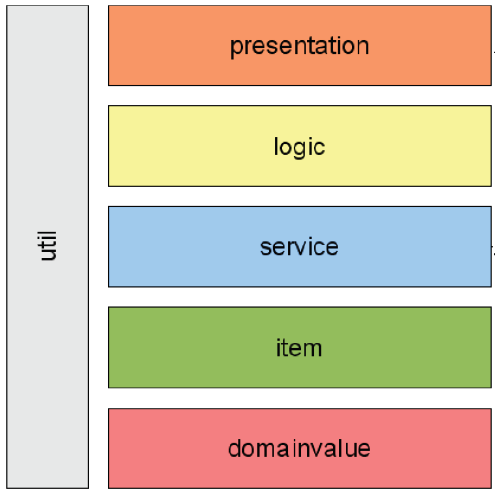
\includegraphics[width=10.5cm]{arch}
  \caption{The given overview of JCommSy architechture}\label{fig:intarch}
\end{figure}
\newpage
\section*{Architecture violations}
\begin{figure}
  \centering
  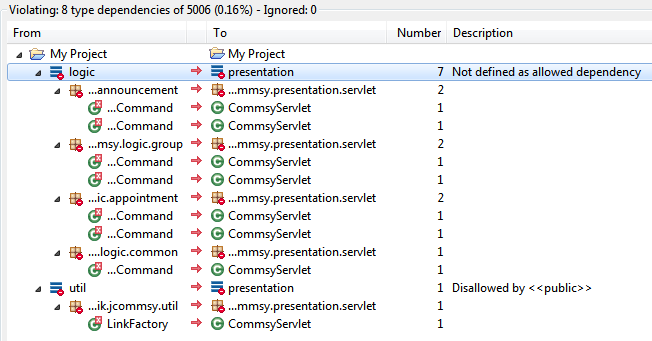
\includegraphics[width=12cm]{archviol}
  \caption{Architecture violations from SonarJ}\label{fig:archviol}
\end{figure}

\section*{Layer Cycles}
\begin{figure}
  \centering
  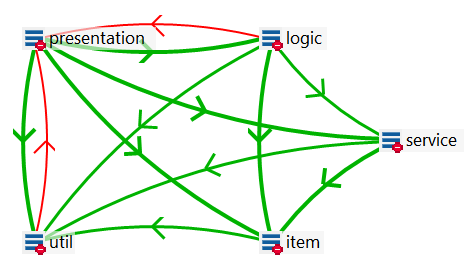
\includegraphics[width=9.5cm]{cycle}
  \caption{Cycles between layers}\label{fig:cycle}
\end{figure}




\end{document}
